\newpage
\section{Apprendimento per rinforzo}

\textit{Gli appunti seguenti sono un riassunto dei punti salienti
del libro di Richard S. Sutton e Andrew G. Barto - Reinforcement
Learning: An Introduction}

L'apprendimento che deriva dall'\textbf{interazione} con un ambiente è una
forma di intelligenza molto comune, la più nota, semplice e intuitiva.

\begin{figure}[H]
\centering
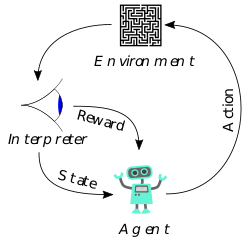
\includegraphics[width=0.4\textwidth]{learning}
\caption{Scenario descrittivo dell'apprendimento per rinforzo}
\end{figure}

L'apprendimento per rinforzo è guidato da un \textbf{obiettivo}, che viene
usato per stabilire se un'interazione con l'ambiente è positiva o negativa.

L'apprendimento per rinforzo consiste nel sapere quale azione intraprendere in
una data situazione, così da massimizzare la \textbf{ricompensa} (di solito
espressa in forma numerica).

Chi apprende attraverso questo meccanismo deve scoprire quali azioni producono
la maggior ricompensa provandole.

La ricerca ``prova, sbaglia, impara'' e la ``ricompensa con slack'' sono due
importanti concetti.\\

Un agente che apprende deve saper riconoscere lo stato dell'ambiente in cui si trova
e interagire con esso in modo tale da cambiarlo. Deve anche sapere qual è
l'obiettivo da raggiungere.

L'apprendimento per rinforzo è diverso sia dall'apprendimento supervisionato
(non dispone di esempi passati che possano dirgli quale sia la cosa giusta
da fare, deve essere in grado di apprendere da se stesso) che dall'apprendimento
non supervisionato (non deve tentare di trovare patterns o strutture in dati
sconosciuti) quello che deve fare, principalmente, è tentare di massimizzare
la ricompensa.

Un agente che apprende deve \textbf{sfruttare} ciò che ha imparato in passato per
ottenere una ricompensa, ma deve anche \textbf{esplorare} nuove azioni per sceglierne
di migliori in futuro.

Questo tipo di approccio permette di gestire le \textbf{incertezze} dell'ambiente in
cui l'agente si trova.

L'effetto di un'azione dell'agente spesso è difficile da prevedere, perciò è necessario
monitorare frequentemente l'ambiente.

(Parentesi psicologica) - tutto ciò si può ricondurre al \textbf{comportamentismo}
(o psicologia comportamentale), un tipo di approccio alla psicologia sviluppato da
John Watson agli inizi del Novecento, basato sull'assunto che il comportamento
esplicito dell'individuo è l'unica unità di analisi scientificamente studiabile della
psicologia avvalendosi del metodo stimolo (ambiente) e risposta (comportamento), in
quanto direttamente osservabile dallo studioso.

\subsection{Elementi del reinforcement learning}

\begin{itemize}
 \item Una \textbf{politica} (mappatura da uno stato dell'ambiente a un'azione da compiere
quando ci si trova in quello stato). Si tratta del cuore di un agente che apprende,
dato che da sola basta per determinarne il comportamento.
 \item Un \textbf{segnale di ricompensa}. Definisce l'obiettivo del problema; a ogni passo
l'agente riceve una ricompensa che deve massimizzare nel lungo termine.
 \item Una \textbf{funzione dei valori}. Mentre la ricompensa definisce ciò che è buono
nel \textbf{breve termine}, la funzione dei valori definisce ciò che è buono nel
\textbf{lungo termine}.
Ne segue che è essenziale quando si devono prendere decisioni/fare delle valutazioni.
Purtroppo i valori sono più difficili da individuare rispetto alla
ricompensa (che è data da uno stimolo dell'ambiente). Di solito occorre osservare tutta
la storia passata di un agente (se disponibile).
Per questo motivo il più importante elemento di un sistema di apprendimento per rinforzo
è proprio quello che effettua la stima dei valori.
Si noti che alcuni sistemi non possiedono una funzione dei valori, ma si basano solo
sulla ricompensa ottenuta e modificano le loro politiche dopo molti tentativi
\textbf{evolvendo nelo tempo}, senza tenere conto delle singole interazioni con l'ambiente
(algoritmi genetici, simulated annealing ecc\dots).
 \item Un \textbf{modello dell'ambiente} (opzionale, visto che può essere completamente
ignoto). Viene usato per fare predizioni sui prossimi stati e ricompense se si effettua una
determinata azione. Tale approccio di pianificazione è considerato opposto alla ricerca
``prova, sbaglia, impara''.
\end{itemize}

I metodi che evolvono le loro politiche non stimano la funzione dei valori e sono utili
in casi in cui un agente non può rilevare lo stato completo dell'ambiente circostante,
mentre i metodi di apprendimento per rinforzo più comuni apprendono interagendo con l'ambiente.

\subsection{K-Bandit Algorithm}

L'apprendimento per rinforzo usa le informazioni di training per valutare le azioni intraprese
piuttosto che decidere qual è l'azione giusta da prendere.

Si suppone di avere a disposizione un set di k azioni e che ciascuna di esse restituisca
una ricompensa quando viene selezionata. L'obiettivo è massimizzare la ricompensa.

L'azione scelta al tempo t è $A_t$ e la corrispondente ricompensa è $R_t$.
Il valore di un'azione arbitraria $a$ è: $q_*(a) = E[R_t | A_t = a]$ cioè il valore atteso
di $R_t$ ogni volta che viene selezionata l'azione $A_t$.

Se si conoscesse $q_*(a)$ allora basteresse scegliere sempre l'azione che restituisce una
ricompensa maggiore. In alcuni casi però si ha a disposizione solo una stima della
ricompensa dell'azione a selezionata al tempo t, detta $Q_t(a)$. Si vorrebbe rendere
$Q_t(a)$ il più possibile vicina a $q_*(a)$.

Le azioni greedy sono quelle che massimizzano $Q_t(a)$. Se vengono selezionate, si sta
sfruttando la concoscenza dell'ambiente, altrimenti se si sceglie di selezionarne altre,
si sta esplorando l'ambiente.

Lo \textbf{sfruttamento} può massimizzare la ricompensa nel breve termine, mentre
l'\textbf{esplorazione} può massimizzarla nel lungo termine.

Ci si può chiedere se queste due strategie siano in conflitto tra loro, ma in realtà
i risultati migliori si ottengono quando vengono bilanciate. Il problema
di bilanciare sfruttamento ed esplorazione è una sfida nell'apprendimento per rinforzo
ed esistono anche tecniche sofisticate.

Un modo di stimare il valore vero delle ricompense è quello di fare la media delle 
ricompense effettivamente ricevute:

\begin{equation}
Q_T(a) = \frac{\sum_{i=1}^{t-1} R_i*Id_{A_i = a}}{\sum_{i=1}^{t-1} Id_{A_i = a}}
\end{equation}

Se il denominatore è 0, allora $Q_t(a)$ assume valore di default 0.
Quando il denominatore tende all'infinito (cioè l'azione a è stata selezionata
infinite volte) allora per la legge dei grandi numeri si è ragionevolmente sicuri che
il numeratore tenda alla media reale, cioè a $q_*(a)$.

Questo metodo di stima dei valori delle azioni è detto \textbf{metodo di campionamento
semplice}.

Il metodo greedy consiste nel selezionare, istante dopo istante, l'azione
$A_t = argmax_a Q_t(a)$ che massimizza la stima dei valori (in caso di pareggio viene
scelta in modo arbitrario tra le azioni alla pari).

Un'alternativa al metodo greedy consiste nel scegliere una volta ogni tanto un'azione
indipendentemente dalla stima con probabilita $\epsilon$. Questo metodo è chiamato
$\epsilon$-greedy.

Il grafico \ref{fig:meanDistributions} mostra i valori reali di $q_*(a)$ per un
problema con 10 possibili azioni e le relative distribuzioni normali (media $q_*(a)$
e varianza unitaria).

\begin{figure}[H]
\centering
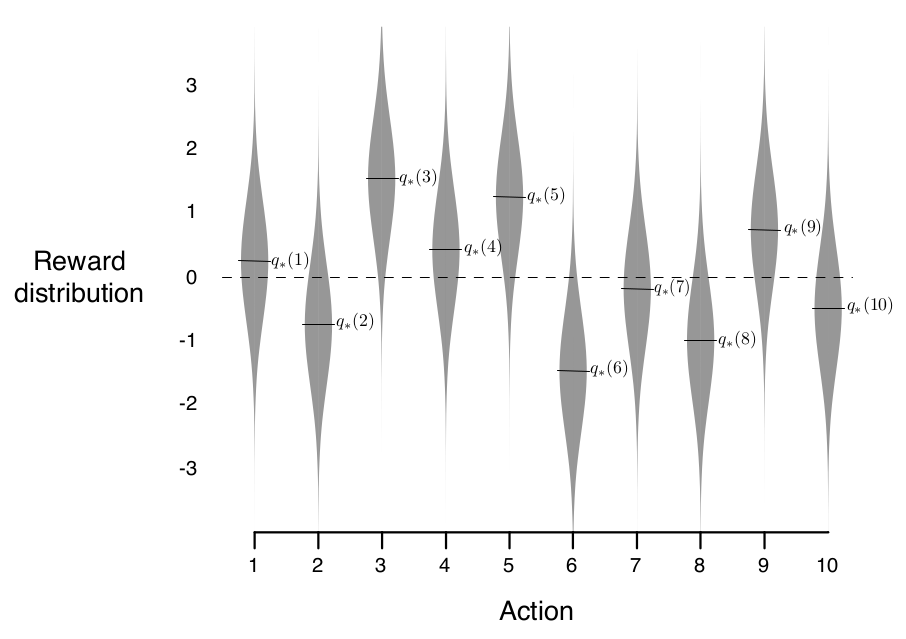
\includegraphics[width=0.6\textwidth]{meanDistributions}
\caption{Distribuzione di $q_*(a)$ per un problema con 10 azioni}
\label{fig:meanDistributions}
\end{figure}

Il grafico \ref{fig:comparison} mostra una comparazione tra un algoritmo
$\epsilon$-greedy (con $\epsilon$=0.01 e $\epsilon$=0.1) e un algoritmo greedy.
Entrambi i metodi hanno stimato i valori di $q_*(a)$ tramite il metodo del
campionamento semplice.

\begin{figure}[H]
\centering
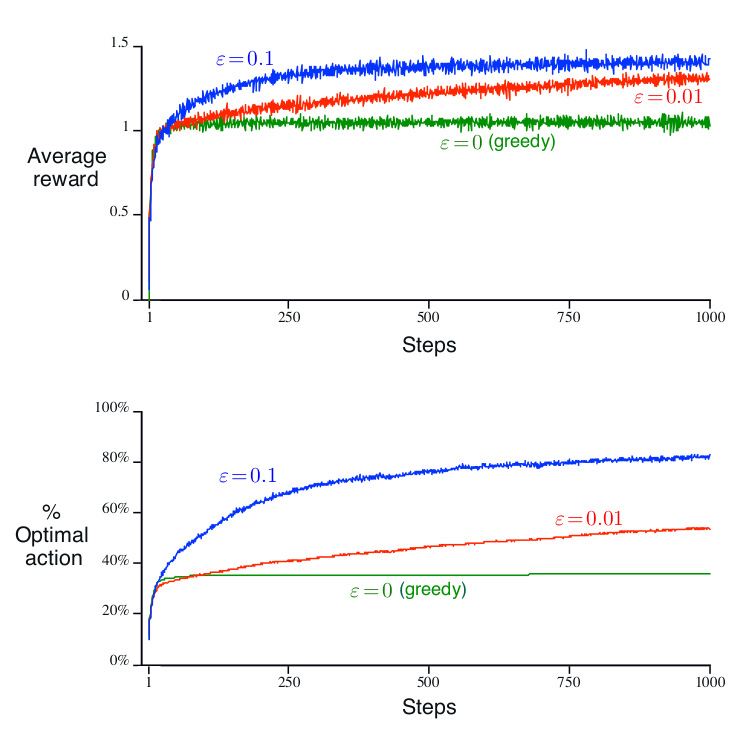
\includegraphics[width=0.6\textwidth]{comparison}
\caption{Comparazione tra un algoritmo $\epsilon$-greedy e un algoritmo greedy}
\label{fig:comparison}
\end{figure}

Una semplice implementazione in python del 10-bandit algorithm è riportata
nel seguente snippet di codice:

\lstinputlisting[language=Python, breaklines=true]{res/code/banditAlgorithm.py}

\subsection{Valori iniziali ottimistici}

In un ambiente non-stazionario, è preferibile che il passo $\alpha$ cambi a ogni
iterazione. Nell'esempio precedente rimane fisso a $\frac{1}{n}$ e permette di convergere
al valore reale delle ricompense delle azioni.

I metodi finora discussi dipendono dalla stima iniziale del valore di
ricompensa delle azioni ($Q_i(a)$).
Per il metodo che utilizza la media come stima di $Q_i(a)$ questo bias
dovuto al valore iniziale viene aggiustato una volta che tutte le azioni
sono state selezionate almeno una volta.

Per un metodo che come passo utilizzi una costante $\alpha$, il bias rimane.
Se decidiamo di dare una stima iniziale di +5 alle ricompense di tutte le
azioni, questa sarà una stima ottimista (in realtà le ricompense reali
segunono una distribuzione normale di probabilità con media 0 e varianza 1).
Cominciare con un valore ottimista (+5) porta il metodo \textbf{puramente}
greedy (con $\epsilon = 0$) ad esplorare di più e avere (\textbf{nel lungo termine})
performances migliori del metodo greedy con stime iniziali a 0 e $\epsilon = 0.01$
(si veda il grafico \ref{fig:greedyOpt}).

\begin{figure}[H]
\centering
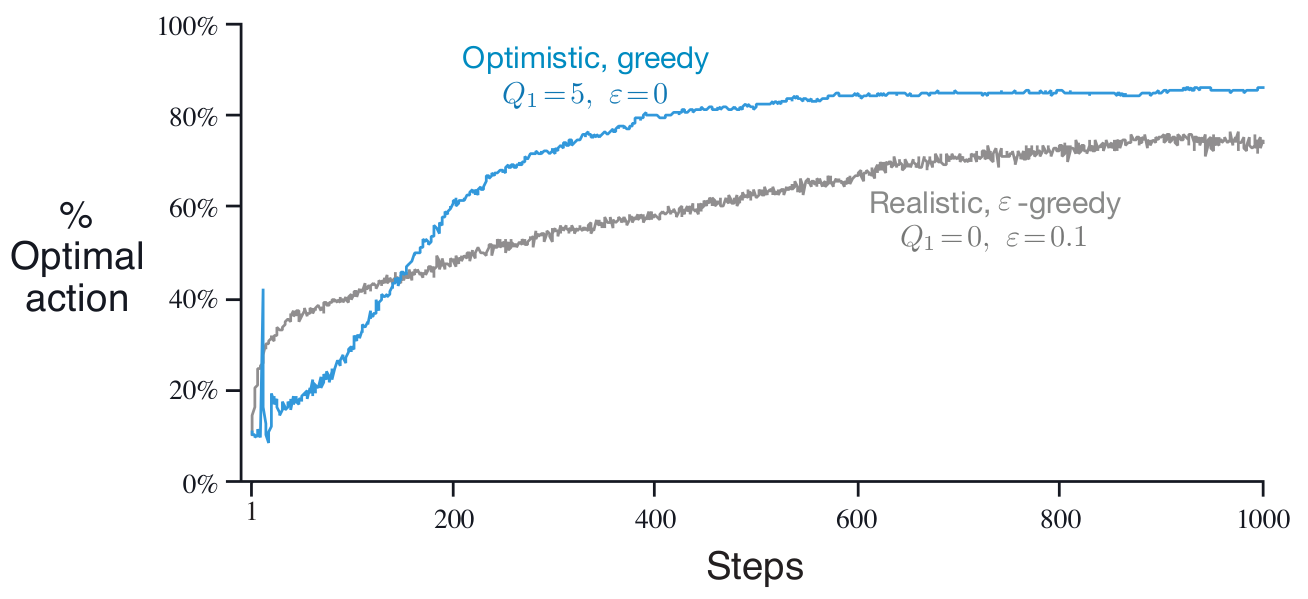
\includegraphics[width=0.6\textwidth]{GreedyOpt}
\caption{Comparazione tra un algoritmo $\epsilon = 0.01$-greedy e un algoritmo
puramente greedy con stime iniziali ottimiste a +5}
\label{fig:greedyOpt}
\end{figure}

\subsubsection{Implementazione incrementale}

Si cerca un'espressione che consenta di ottimizzare il calcolo della stima della reward di un'azione,
possibilmente in tempo costante.
Calcolare ogni volta la media con la formula usuale non è efficiente:

\begin{equation}
 $Q_1 := \frac{R_1 + R_2 + ... + R_n}{n - 1}$
\end{equation}

conviene sfruttare la media calcolata fino al passo precedente ($Q_{n-1}$) per calcolare la
nuova, tramite la formula:

\begin{equation}
 $Q_n := Q_{n-1} + \frac{1}{n}[R_n - Q_n]$
\end{equation}

La precedente formula viene generalizzata in:

\begin{equation}
 $Nuova stima <- vecchia stima + passo[target + vecchia stima]$
\end{equation}

L'espressione $passo[target + vecchia stima]$ è un errore della stima (tra la vecchia
e la nuova).

Il $passo$ cambia di volta in volta.


\subsection{Selezione basata sull'upper confidence bound}

Come scegliere le azioni nel caso non greedy in modo più proficuo
rispetto alla casualità? Lo scopo è quello di esplorare con qualche indicazione
in più, o comunque in modo più intelligente rispetto a quello random.

Un modo è quello di selezionare, al tempo t, l'azione $A_t$:

\begin{equation}
A_t = argmax_a [Q_t(a) + c \sqrt{\frac{ln t}{N_t(a)}}]
\end{equation}

dove c rappresenta il \textbf{grado di esplorazione} e il termine
sotto la radice indica l'incertezza relativa alla stima $Q_t(a)$.

Quello che si fa è massimizzare l'upper bound della possibile
ricompensa reale di un'azione a. Il tempo è usato come un
indicatore della stima: se un'azione viene selezionata molte volte,
la stima della sua ricompensa migliora e l'incertezza diminuisce,
se non viene selezionata per molto tempo la stima della sua
ricompensa peggiora e l'incertezza aumenta.
Questo metodo non funziona molto bene in casi generali o in problemi
non-stazionari. Comunque, nel problema del k-Bandit funziona bene
come si può dedurre dal grafico \ref{fig:ucb}

\begin{figure}[H]
\centering
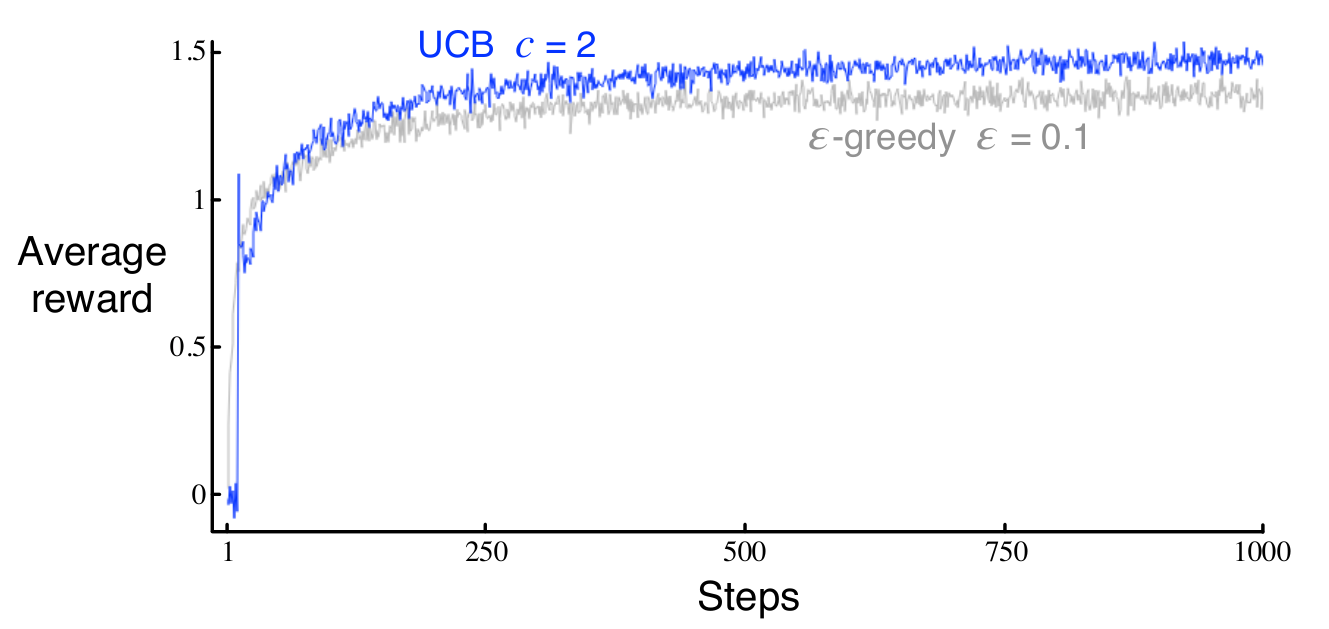
\includegraphics[width=0.6\textwidth]{ucb}
\caption{Comparazione tra un algoritmo $\epsilon = 0.01$-greedy e un algoritmo
che seleziona l'azione con il criterio ucb (c = 2)}
\label{fig:ucb}
\end{figure}



